\chapter{Experiments: Squeezed Light}
This chapter will cover the experimental methods used in the development of frequency-dependent squeezing in optomechanical systems, focusing on the generation of squeezed light, optical locking techniques, and quadrature measurement methods. The methods are designed to enhance the sensitivity of measurements in quantum optics and optomechanics.
\minitoc
\newpage 

\section{Optical Setup Overview}

The generation and manipulation of squeezed light is a complex process that requires a carefully designed optical setup. Over the course of \textbf{Sheon CHUA} postdoctoral work at the lab, \textbf{Michael CROQUETTE} PhD work, and my own PhD work, we have developed a versatile setup aiming at producing both bright and vacuum squeezed states of light using an Optical Parametric Oscillator (OPO) below threshold. Squeezing experiments being very prone to losses, noises, or any type of imperfection, the optical table is protected from air currents and temperature fluctuations using a custom-made cabin (inspired from the lab of \textbf{Julien LAURAT} and \textbf{Alban URVOY}), and the optics were initially mounted in two boxes such that they could be transported easily between different labs, or stacked on top of each other to save space (inspired from \textbf{Roman SCHNABEL} lab). Pictures of the setup are shown in \\

\begin{figure}[h!]
    \centering  
    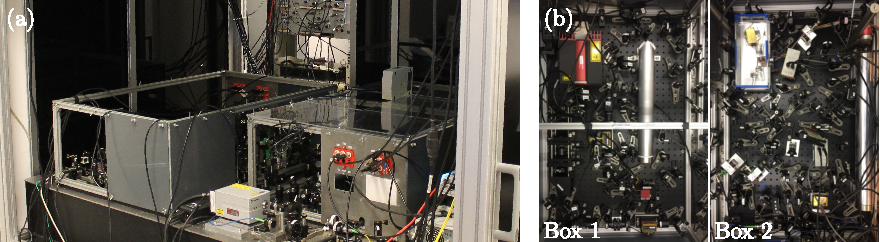
\includegraphics[width=\textwidth]{./chap6/fig/manipssqz.pdf}
    \caption{Pictures of the optical setup for squeezed light generation and detection. (a) Overview of the experiment inside the cabin. (b) Top view of the two boxes containing the optics for squeezed light generation and detection.}
    \label{fig:opticalpath}
\end{figure}


We first provide a general overview of the optical setup used to generate and manipulate squeezed light. 
Two lasers are used in this setup, to give flexibility as to produce bright squeezing directly from the OPO (one laser only), or produce vacuum squeezing to be mixed with a bright coherent field (two lasers). Both lasers are 1064nm Nd:YAG lasers (Coherent Mephisto and Mephisto S) as in the previous chapter. The full optical layout is shown in figure \ref{fig:opticalpath}. The dashed box on the right part of the squeezing setup is the one to be changed to implement both configurations, as shown in figure \ref{fig:configsqueezer}. The experiment was designed as to easily switch between the two configurations. Throughout this chapter, we will refer to three different optical cavities common to the two configurations: the infrared mode cleaner (IRMC) cavity, the SHG cavity, and the OPO cavity. Each of these cavities is central to the generation and manipulation of squeezed light, and their characterization is detailed in the following sections. \\ 

\begin{figure}[h!]
    \centering  
    \includegraphics[width=\textwidth]{./chap6/fig/schemaSqz.pdf}
    \caption{Optical layout for squeezed light generation and detection. The setup includes two Nd:YAG lasers, an IRMC cavity for spatial filtering, a SHG cavity to produce the pump beam at 532 nm, and an OPO cavity for squeezing generation. The homodyne detection setup is used to measure the squeezed states. Key components such as electro-optic modulators (EOMs), piezoelectric transducers (PZTs), and photodiodes (PDs) are indicated for locking and detection purposes.}
    \label{fig:opticalpath}
\end{figure}

To generate bright squeezed light from an OPO, we now detail the two different configurations implemented in this setup, as shown in figure \ref{fig:configsqueezer}. The only notable modification between the two configurations lies in the way the OPO is seeded and locked, and in what the piezo actuators are used for. 

\begin{figure}[h!]
    \centering  
    \includegraphics[width=\textwidth]{./chap6/fig/config_squeezer.pdf}
    \caption{Schematic of the two configurations for squeezed light generation. (a) Configuration I: bright squeezing from OPO using a single laser source. The IR beam from the IRMC cavity is split into two paths: one for the local oscillator (LO) and one as a bright seed for the OPO. (b) Configuration II: vacuum squeezing with a bright seed using two lasers. The first laser serves as the detection LO and bright coherent state, while the second laser provides a bright coherent field detuned from the OPO resonance. The outputted vacuum squeezing is then mixed with the bright seed to generate bright squeezing.}
    \label{fig:configsqueezer}
\end{figure}


\subsubsection{Configuration I: bright squeezing from OPO} The first one uses a single laser source, where the main laser beam is split into two paths. It is shown in figure \ref{fig:configsqueezer}(a). The IR beam outputted from the IRMC cavity is split in two paths: one path is the LO used in the detection, while the other one is sent to the OPO as a bright seed. Locking the pump phase then allows to select the squeezed quadrature. The piezo shown is then used to lock the LO phase. 

\subsubsection{Configuration II: vacuum squeezing + bright seed} The second configuration employs the two lasers. Its schematic configuration is shown in figure \ref{fig:configsqueezer}(b). The first laser is used both as a detection LO, as well as a bright coherent state to be mixed with the squeezed vacuum generated by the OPO. In this case, the piezo shown is used to lock the the relative phase between the bright seed and the vacuum squeezing ellipse angle as to select the squeezed quadrature. A second piezo not displayed here is used to lock the signal quadrature to be probed by the detection. The second laser provides a brigth coherent field detuned from the OPO resonance. This field, seen as a strong sideband, is injected into the OPO cavity. The photons generated from the pump beam at 532nm will then be down-converted into pairs of photons, which eventually populate the sideband mode at the second laser frequency. These correlated photons being equally distributed in the upper and lower sidebands around the first laser frequency (since the pump was generated from it), demodulating the IR signal leaking from the cavity at the PLL frequency and twice the PLL frequency allows to extract two error signals. The first one, at the PLL frequency, give us the phase of the phase of the pump with respect to the bright seed, while the second one, at twice the PLL frequency, gives us access to the quadrature angle of the squeezed vacuum with respect to the bright seed. Hence, we lock the pump phase using the first error signal, while the second error signal is used to lock the homodyne angle to the optimal squeezing quadrature. \\ 

The second configuration is more complex to implement, but is meant to render the squeezing generation more robust to low-frequency noises. It was studied over Michael Croquette's PhD thesis \cite{croquette_thesis} and the start of mine, where we obtained 3dB of vacuum squeezing and 1.5dB of bright squeezing. These results will quickly be summarized in section \ref{sec:bright_squeezingII}, but we will mainly focus on the first configuration in the rest of this chapter \ref{sec:bright_squeezingI}, as it is simpler to implement and optimize. 

\section{Cavity Resonances and Locks}

\subsection{IRMC Cavity}
The first cavity presented is the infrared mode cleaner (IRMC) cavity. The purpose of this cavity is to spatially filter the laser beam, ensuring a high-quality TEM00 mode profile, as well as \textit{cleaning} the IR beam from any excess classical noise as developped in Chapter I. It is a three mirror - \textit{travelling wave} Fabry-Pérot resonator with a total round-trip length of $L = 84$ cm, corresponding to a free spectral range of $\mathrm{FSR} = 357$ MHz. The input and output coupler have a radius of curvature of $\mathrm{RoC} = -2$ m, while the middle mirror is flat. With a measured optical linewidth of $\kappa/2\pi = 52$ kHz, the finesse reaches a value of $\mathcal{F} \sim 7000$, which ensures significant filtering of laser frequency noise and intensity noise above the cavity linewidth. The associated round-trip losses are estimated to be around $900$ ppm, dominated by the input coupler transmission of $T_1 = 666$ ppm. The cavity parameters are summarized in Table \ref{tab:IRMC params}. \\

\begin{table}[h!]
    \centering
    \captionsetup{width=0.55\linewidth}
    \begin{tabular}{lc}
        Specifications &  \\
        \hline
        Length (cm)              & 84.0 \\
        FSR (MHz)                  &  357 \\ 
        $T_1^{\text{spec}}$ (ppm) & 475 \\
        $T_2^{\text{spec}}$ (ppm) & 475 \\
        RoC (m) & -2 \\[0.6em]

        Measurements &  \\
        \hline
        Finesse $\mathcal{F}$& 6812 \\
        Linewidth (kHz)            & 52 \\
        $T_1 + T_2 + \mathcal{L}$ (ppm) & 922  \\
        Resonant reflection R(0) & 0.44 \\
        $T_1$ (ppm) & 767 \\
        $T_2 + \mathcal{L}$ (ppm) & 155 \\[0.6em]

    \end{tabular}
    \caption{IRMC parameter table summary.}
    \label{tab:IRMC params}
\end{table}

This cavity is mounted in a aluminium housing to make it as monolitic as possible. The optimal alignment of the cavity is found by first making sure the laser beam goes through the first two mirrors without being clipped. This is most easily done by positioning a IR camera in transmission of the cavity rather than a photodiode. Once the beam is well centered on the first two mirrors, we adjust the angle of the output coupler to center the beam on the concave/second mirror. We then adjust the position of the concave mirror such that the first reflection spot coincides with the input beam on the input coupler surface. Finally, we adjust the angle of the input coupler to superpose the consecutive round-trip spots with the input beam reflected from the input coupler surface. This is most easily done in the far-field limit, such that great angular precision can be achieve doing so. A characteristic elliptic shape formed by the multiple spots appears as one converges to the optimal alignment, seen both in reflection on an IR card and in transmission on the IR camera. Once the cavity is pre-aligned, we position a photodiode in both reflection and transmission of the cavity, and scan the cavity length. One can then beam walk the input beam as to maximise the coupling to the TEM00 mode of the cavity, observed as the highest and narrowest resonance peak in transmission. Triggering the oscilloscope on the PZT ramp, we measure the cavity linewidth and finesse, as well as the resonant reflection to estimate the various cavity parameters. \\

The cavity is then locked using a standard PDH technique, with a preliminary side-of-fringe lock to bring the cavity close to resonance. The input beam is phase-modulated at $\Omega_\mathrm{mod} = 21$ MHz using a free space EOM (New Focus IR 4003). The cavity length is swept, and the detected reflected beam is manipulated with PyRPL to generate the PDH error signal. The finesse being relatively high, we observed cavity ringing effects when scanning the cavity length resonance too quickly, as already seen in the previous chapter. The cavity length was then swept over gently at 0.5 Hz as to recover the expected lorentzian resonance peaks in reflection. \\

Once locked, the intensity noise spectra of the reflected and transmitted beam are measured in direct detection. We then renormalize the transmitted spectra by the known $R(0)$ to yield equivalent optical powers. The results are shown in figure \ref{fig:irmcnoise}, where we observe significant noise suppression above the cavity bandwidth (half linewidth) of $26$ kHz. This is notably seen in the attenuation of the laser relaxation oscillation peak around $1$ MHz. However, at low frequencies, the intensity noise is amplified, most likely due to the feedback loop. Above 2 MHz, the intensity noise reaches the shot noise level, indicating that the IRMC effectively filters classical intensity noise from the laser. At the membrane fundamental mode frequency of $\sim$ 850 kHz, the laser intensity noise is suppressed by approximately 20 dB, which is beneficial for optomechanical experiments. It does however not reach the shot noise level, indicating that further improvements in the cavity locking or laser stabilization may be necessary for optimal performance. \\

\begin{figure}[h!]
    \centering  
    \includegraphics[width=\textwidth]{./chap6/fig/NoiseIRMC.pdf}
    \caption{Noise spectra of the IRMC transmitted beam in direct detection, showing significant suppression of classical intensity noise above the cavity linewidth. We show the curves for unfiltered IR beams with and without the laser noise eater on, where we see the relaxation oscillation peak being significantly attenuated and shifted up in frequency when the noise eater is on. The relaxation oscillation peak around 1 MHz is notably attenuated upon IRMC filtering. However, low-frequency noise is amplified, likely due to feedback effects. Above 2 MHz, the intensity noise reaches the shot noise level, indicating effective filtering of classical noise by the IRMC.}
    \label{fig:irmcnoise}
\end{figure}

The IRMC beam is now directed to the homodyne detection setup to measure the phase noise of the transmitted beam. The results are shown in figure \ref{fig:noiseLO}, where we observe a linear variation of the phase noise with the LO power, confirming that the detected noise is indeed shot noise limited. The residual classical noises below 2 MHz are effectively killed by the HD detection, and we deduce a clearance of approximately 10dB up to 10 MHz, which is satisfactory for squeezing measurements.

\begin{figure}[h!]
    \centering  
    \includegraphics[width=\textwidth]{./chap6/fig/NoiseLO.pdf}
    \caption{Noise spectra of the IRMC transmitted beam in homodyne detection, showing shot noise limited behavior across the measured frequency range. The phase noise scales linearly with the LO power, confirming the shot noise dominance. A clearance of approximately 10 dB is observed up to 10 MHz, indicating effective suppression of residual classical noise by the homodyne detection scheme.}
    \label{fig:noiseLO}
\end{figure}


\subsection{SHG Cavity}

In order to generate a stable $532\,\mathrm{nm}$ pump beam for the OPO, we implemented and characterized a linear SHG cavity. The cavity is designed to resonantly enhance an incoming IR field at $1064\,\mathrm{nm}$, and convert it to its second harmonic at $532\,\mathrm{nm}$ using a periodically poled lithium niobate (PPLN) crystal as the nonlinear medium. The crystal is a Covesion $1\times10\times10$mm$^3$ MgO:PPLN SHG crystal with five different quasi-phase-matching gratings in the bulk, with poling periods ranging from $6.83\,\mu\mathrm{m}$ to $6.96\,\mu\mathrm{m}$ and apertures of 1mm$^2$. The crystal is temperature controlled using a Covesion\textsuperscript{\textregistered} temperature controller to achieve optimal phase matching for SHG, with a temperature stabilized to 10mK precision. The crystal and its oven are then positioned at the center of the SHG cavity. The cavity features two mirrors with radii of curvature -250mm, ensuring that the crystal length is shorter than the Rayleigh range of the cavity mode, thus minimizing diffraction losses. The output coupler is HR coated for both IR and green wavelengths, while the input coupler has a transmission of 10\% at $1064\,\mathrm{nm}$ and less than 1\% at $532\,\mathrm{nm}$. These characteristics are summarized in table \ref{tab:SHG params}. It results in a theoretical cavity finesse of approximately $60$ at $1064 \, \text{nm}$, while the finesse at $532 \, \text{nm}$ would be around $1$, as no cavity buildup is desired at this wavelength. The reflected IR and green beams are then seperated on a dichroic mirror before being sent to their respective detection systems, as seen in figure \ref{fig:shglock}(a). \\ 

\begin{table}[h!]
    \centering
    \captionsetup{width=0.55\linewidth}
    \begin{tabular}{lc}
        Specifications &  \\
        \hline
        Length (cm)              & 9 \\
        FSR (GHz)                  &  3.3\\
        Specified $T_1$ @1064nm & 10\% \\
        Specified $T_2$ @1064nm & 0.5\% \\
        Specified $T_1$ @532nm & >99\% \\
        Specified $T_2$ @532nm & <0.1\% \\
        Roc input/output (mm) & -250 \\[0.6em]
        Measurements &  \\
        \hline
        Finesse IR $\mathcal{F}$& 30 \\
        Linewidth (MHz)            & 111  \\ 
        $T_1 + T_2 + \mathcal{L}$ (ppm) & $\sim 2.10^6$  \\
    \end{tabular}
    \caption{SHG cavity parameter table summary. The specified values are taken from the PhD thesis of M. Croquette \cite{croquette_thesis}.}
    \label{tab:SHG params}
\end{table}

This cavity is first aligned without the crystal to find the optimal cavity mode. Taking off the input coupler, we center the beam on the output coupler, and adjust its angle to retro-reflect the beam back onto itself, using two irises for example. We then re-insert the input coupler and adjust its angle to superpose the input beam with the retro-reflected beam from the output coupler. Once the cavity is pre-aligned, we insert the PPLN crystal and adjust its position to recover the cavity resonance peaks, as well as placing a photodiode in transmission to monitor resonances on an oscilloscope. One can then beam walk the input beam as to maximize the coupling to the TEM00 mode of the cavity, observed as the highest and narrowest resonance peak in transmission. Doing so, and if the IR beam passes through one of the PPLN gratings (and not in between), we observe green flashes by eye, indicating successful SHG every time the cavity comes to resonance. \\ 

Initial characterization was performed by scanning the cavity length around resonance using a piezoelectric transducer on which the cavity output coupler was glued. The input infrared power was maintained at approximately $100\,\mathrm{mW}$. The transmitted IR signal and the generated green output were simultaneously monitored on fast photodiodes. Typical traces of the transmitted IR beam are shown in Fig.~\ref{fig:shglock}(b)–(c). As the cavity length is swept, the cavity exhibits sharp IR resonance peaks, corresponding to successive TEM00 modes of the cavity. At the same time, the green output rises only in coincidence with infrared resonances, confirming that efficient SHG occurs exclusively under resonant build-up of the fundamental field. The actual IR finesse was measured to be $\mathcal{F} = 30 $, where the discrepancy is attributed to poor knowledge of the mirror parameters, as well as optical losses from the non linear medium. The polarization of the input beam is controled by half and quarter waveplates as to maximize the output green power, and the symmetry of the resonance peaks in the scans further indicates negligible birefringence in the PPLN crystal. \\

This cavity is first aligned without the crystal in order to identify the optimal cavity mode. After removing the input coupler, the beam is centered on the output coupler and its angle is adjusted to retro-reflect the beam back onto itself (e.g., using two irises). The input coupler is then re-inserted and aligned so as to overlap the incident beam with the retro-reflected beam from the output coupler, providing a robust pre-alignment of the cavity. The PPLN crystal is subsequently inserted and its position is adjusted to recover the cavity resonances, while a transmission photodiode is used to monitor the resonance peaks on an oscilloscope. Final coupling is optimized by beam-walking the input beam to maximize the TEM${00}$ coupling, identified as the highest and narrowest transmission resonance; when the infrared beam is correctly routed through one of the PPLN gratings (and not between gratings), green flashes are observed at resonance, indicating efficient SHG. Initial characterization is then performed by scanning the cavity length around resonance using a piezoelectric transducer bonded to the output coupler, while maintaining an input infrared power of approximately $100,\mathrm{mW}$. The transmitted infrared signal is monitored on a fast photodiode (see typical trace in Fig.~\ref{fig:shglock}(b)), showing sharp infrared resonance peaks with green output occurring only in coincidence with these resonances, consistent with SHG taking place exclusively under resonant build-up of the fundamental field. The infrared finesse is measured to be $\mathcal{F}{\mathrm{IR}}=30$, with the discrepancy attributed to imperfect knowledge of the mirror parameters and additional intracavity losses introduced by the nonlinear medium. The input polarization is adjusted using half- and quarter-waveplates to maximize the generated green power, and the observed symmetry of the resonance peaks further suggests negligible birefringence in the PPLN crystal. \\ 


\begin{figure}[h!]
    \centering  
    \includegraphics[width=\textwidth]{./chap6/fig/SHGlock_sweep.pdf}
    \caption{Overview of the SHG cavity locking: (a) Schematic of the PDH lock setup used to stabilize the SHG cavity length to resonance. The temperature of the PPLN crystal is locked via a commercial temperature controller from Covesion \textsuperscript{\textregistered}. (b) Cavity scan at low input IR power, showing the IR resonances onto which the cavity is locked. A PDH error signal, not displayed here, is tuned as to lock the cavity (c) Cavity lock as seen on the scope, showing the transmitted IR power (red) and the generated green power (green). We observe a drift away from the nominal peak height, due to thermal effects in the crystal. More precisely, the heating of the crystal changes the effective optical length of the cavity, hence shifting the resonance condition. This needs to be tuned by the experimenter. 
     }
    \label{fig:shglock}
\end{figure}


Modulating the input IR beam at $\Omega_\mathrm{mod} = 21\,\mathrm{MHz}$ using the same free space EOM as for the IRMC cavity (New Focus\textsuperscript{\textregistered} IR 4003), we manipulated the detected IR signal into a PDH error signal suitable for locking the cavity length to resonance, with a preliminary side-of-fringe lock as usual. A typical lock trace is shown in Fig.~\ref{fig:shglock}(c), where both the transmitted IR power and the generated green power are monitored on an oscilloscope. The first striking observation is the drift of the transmitted IR and reflected green power away from their nominal peak heights. This effect is attributed to thermal effects in the PPLN crystal: upon locking, the intracavity IR power stabilizes at a relatively high intensity, leading to heating of the crystal due to residual absorption. This heating causes a change in the refractive index and physical dimensions of the crystal, thereby shifting the optimal quasi phase matching temperature (the oven would need to be locked to a lower temperature as to compensate for this extra optical heating). As a result, the cavity drifts away from the optimal resonance, necessitating a manual tuning of the temperature setpoint to recover maximum green output. Keeping the IR power at about 200mW, we could then scan the crystal temperature to find the optimal phase-matching condition for SHG. The results are shown in Fig \ref{fig:shgtemp}(a), where we found a maximum green output of around $100\,\mathrm{mW}$ at a crystal temperature of $\sim 58^{\circ}\mathrm{C}$ for the $6.90\,\mu\mathrm{m}$ grating, sufficient to pump the OPO below threshold. The conversion efficiency usually follows a sinc-squared dependence on temperature. Due to the high IR power build-up in the cavity, thermal effects are observed, which distort the expected sinc$^2$ shape as reported in ...The side lobes of the sinc$^2$ curve are seen when scanning th temperature over a larger range, but we only show the central peak here. The symmetric sinc$^2$ shape is however recovered when injecting an order of magnitude less IR power, but not useful to our purpose as it does not provide sufficient power for the OPO. To measure our SHG conversion efficiency, we varied the input IR power while keeping the crystal temperature at the optimal phase-matching point by tuning the temperature slightly at each new IR power injected to maximise the output green power. The results are shown in Fig \ref{fig:shgtemp}(b), where we observe a pseudo-linear dependence of the green output power with respect to the input IR power. From a linear fit, we extract a conversion efficiency of approximately $54\%$, which is (very) satisfactory for our application, and rather high compared to similar setups in the literature \cite{eckardt_high-efficiency_2019, kourogi_high-efficiency_2020}. \\ 

\begin{figure}[h!]
    \centering  
    \includegraphics[width=\textwidth]{./chap6/fig/SHGscansTemp.pdf}
    \caption{Output power of the SHG cavity varying against different parameters: (a) Output green power measured against the crystal temperature, showing the phase-matching curve at high input IR power. A histerisis is observed due to thermal effects. (b) Output green power as a function of the IR input power, showing pseudo linear behavior. The SHG conversion efficiency is extracted from a linear fit, yielding a value of $54 \%$}
    \label{fig:shgtemp}
\end{figure}


We can now place a photodiode on the path of the outgoing green beam to monitor its intensity noise spectrum. The results are shown in figure \ref{fig:shgnoise}, where we observe significant excess intensity noise above the shot noise level for frequencies in the range Hz-10MHz. We identify the peak at 2MHz as the relaxation oscillation frequency of the IR laser transduced to the second harmonics field. This excess noise will severly limit the achievable squeezing level from the OPO, as classical pump noise is known to degrade squeezing generation. We can however expect to achieve squeezing above the 2MHz band. \\ 

\begin{figure}[h!]
    \centering  
    \includegraphics[width=\textwidth]{./chap6/fig/NoiseSHG.pdf}
    \caption{Intensity noise spectrum of the SHG output beam, showing significant excess noise above the shot noise level across the measured frequency range. The relaxation oscillation peak at 2 MHz is notably transduced from the fundamental IR laser to the second harmonic field, indicating that classical pump noise may limit squeezing performance in the OPO. The noise floor is not the same as for the previous figure because the RBW is different. }
    \label{fig:shgnoise}
\end{figure}



We now have a \textit{clean} TEM00 IR beam from the IRMC cavity outputting up to 200mW, as well as a stable TEM00 532nm green pump beam from the SHG cavity delivering up to 200mW. Both beams are now directed to the OPO cavity for squeezing generation. Further improvements of the experimental setup could include a Mach-Zehnder (MZ) interferometer after the SHG cavity to stabilize the green power sent to the OPO, as thermal effects in the PPLN crystal can lead to fluctuations in the output power over time [ref], as well as a mode cleaner cavity for the green beam too, to ensure a high-quality spatial mode and suppress any classical noise from the SHG process and cavity locking. However, these improvements were not implemented in the current setup, and it is thought that these would alter the (relative) simplicity of the setup without significantly lowering classical noises. 

\subsection{OPO Cavity}
The final cavity is the Optical Parametric Oscillator (OPO) cavity, which is the core of the squeezed light generation setup. The OPO is bow-tie travelling-wave cavity designed to be resonant for both the fundamental IR field at $1064\,\mathrm{nm}$ and the pump field at $532\,\mathrm{nm}$. The cavity contains a periodically poled potassium titanyl phosphate (PPKTP) crystal as the nonlinear medium for parametric down-conversion. The crystal is a Raicol\textsuperscript{\textregistered} $1\times5\times11.2$ mm$^3$ PPKTP crystal with a poling period of $9.0\,\mu\mathrm{m}$, designed for type-I phase matching at room temperature. It has been coated on both sides to be anti-reflective at both $1064\,\mathrm{nm}$ and $532\,\mathrm{nm}$ by Laseroptik\textsuperscript{\textregistered}, and is mounted in a temperature-controlled oven to maintain phase-matching conditions, with a temperature stability of 100mK. The crystal further features a wedge angle on one face to allow for gross tuning of the quasi-phase-matching condition by displacing the crystal using the 4 axis mount the whole assembly is held on (Newport\textsuperscript{\textregistered} 9071-M). The fine tuning of the phase-matching is achieved by adjusting the crystal temperature. \\

The cavity is formed by two concave mirrors with a radius of curvature of $25\,\mathrm{mm}$, as well as two flat mirrors. One of the flat mirrors is mounted on a PZT actuator to allow for cavity length tuning and locking. The angle of the bow tie cavity needs to be as small as possible to optimize the mode matching (reduces astigmatism), while keeping a sufficient distance between the mirrors to accommodate the crystal mount. To align the cavity, we follow a similar procedure as for the IRMC cavity (and any travelling wave cavity for that matter). Using the pump beam as a proxy (because seeable with the eye), we first center the beam on the first two (flat) mirrors without clipping, then adjust the angle of the second mirror to center the beam on the first concave mirror. We similarly ajust the position of this mirror to center the beam on the second concave mirror, and then adjust its angle to reflect it onto the input beam spot on the input coupler surface. Finally, we adjust the angle of the input coupler to superpose the consecutive round-trip spots with the input beam reflected from the input coupler surface, once again in the far-field limit for better precision (and watch out for that typical elliptical shape). Once the cavity is pre-aligned, we position a photodiode in both reflection and transmission of the cavity, and scan the cavity length. One can then beam walk the input beam as to maximise the coupling to the TEM00 mode of the cavity as usual. We then insert back the crystal mount and adjust its position to recover the cavity resonance peaks. This step can be very tricky and time-consuming, as the crystal mount can easily clip the beam if not well centered. Injecting the IR beam from the IRMC output, we then beam walk the input beam to maximize the coupling to the TEM00 mode of the cavity. To achieve co-resonance, we then proceed to the gross tuning of the quasi-phase-matching condition by displacing the crystal laterally using the 4 axis mount while scanning the cavity length, by periodically beam walking the two beams to remain optimally matched to the fundamental mode. We can then proceed to the cavity characterization. \\

The mirror coatings of the OPO cavity were selected with the primary objective of maximizing the escape efficiency of the squeezed field at 1064\,nm, while maintaining a pump resonance at 532\,nm that is sufficiently robust for stable operation. As seen before in chapter I, this motivates an overcoupled design at 1064\,nm, in which the desired output coupler dominates the total round-trip dissipation. Writing the effective round-trip loss rate for the down-converted field as the sum of the output coupling and parasitic losses, we recall the definition of the escape efficiency $\eta_{\mathrm{esc}}$:
\begin{equation*}
\eta_{\mathrm{esc}}
= \dfrac{\kappa_{2}}{\kappa} = \frac{T^{1064}_{2}}{T^{1064}_{2} + T^{1064}_{1} + \mathcal{L}},
\label{eq:eta_esc_def}
\end{equation*}
where $T^{1064}_{1}$ is the power transmittivity of the 1064\,nm output coupler and $\mathcal{L}$ denotes the additional loss. Experimentally, we measured $T^{1064}_{\mathrm{out}} + \mathcal{L} \simeq 7.5\%$. Assuming additional losses on the order of a few hundred ppm, we get an estimated escape efficiency of $\eta_{\mathrm{esc}} \approx 99.2\%$. \\ 

On the pump side (532\,nm), the coating strategy is intentionally different. The pump resonance was designed to be low finesse ($\mathcal{F}_{532}\approx 8.5$) with a large pump input coupler ($T^{532}_{\mathrm{in}}\approx 74\%$). A broad pump resonance improves operational robustness by reducing sensitivity to cavity-length fluctuations and simplifying acquisition and locking, while still enabling sufficient circulating pump power to reach threshold (measured $P_{\mathrm{th}}\approx 80\,\mathrm{mW}$). It however jitters the coresonance, seen as abrupt variations of the seed amplification/deamplification traces, too fast to be corrected by the temperature control. Overall, the combined coating choices implement a consistent design philosophy: \textit{minimize parasitic loss and enforce overcoupling at 1064\,nm to maximize escape efficiency and preserve squeezing}, while \textit{keeping the pump resonance forgiving and efficiently driven at 532\,nm to ensure stable, reproducible operation}. The measured parameters of the OPO cavity are summarized in Table \ref{tab:OPO params}. \\

\begin{table}[h!]
    \centering
    \captionsetup{width=0.55\linewidth}
    \begin{tabular}{lc}
        Specifications &  \\
        \hline
        Length (cm)              & 27.2 \\
        FSR (GHz)                  &  1.1\\
        RoC (mm) & -38 \\[0.6em]

        Measurements &  \\
        \hline
        IR Finesse $\mathcal{F}_{1064}$& 84 \\
        IR Linewidth (MHz)            & 13  \\
        IR resonant reflection R$^\text{1064}$(0) & 0.97 \\
        IR input coupler $T_1^{\text{1064}}$ & 0.02\%\\
        IR output coupler $T_2^{\text{1064}} + \mathcal{L}$ & 7.5\% \\[0.6em] 

        Pump Finesse $\mathcal{F}_{532}$& 8.5 \\
        Pump Linewidth (MHz)            &  130  \\
        Pump resonant reflection R$^{532}$(0) & 0.87 \\
        Pump input coupler $T_1^{532}$ & 74\% \\
        Pump output coupler $T_2^{532} + \mathcal{L}$ & 3\% \\[0.6em]

        OPO threshold P$_{\text{th}}$ & 80.2 mW \\
        escape efficiency & 99.2\% \\ 
    \end{tabular}
    \caption{OPO cavity parameter table summary.}
    \label{tab:OPO params}
\end{table}



The cavity length is now swept using the PZT actuator to observe the resonances at both wavelengths. The input pump beam is phase-modulated at $\Omega_\mathrm{mod} = 19\,\mathrm{MHz}$ (New Focus\textsuperscript{\textregistered} IR 4001), and the transmitted and reflected signals are manipulated with PyRPL to generate a PDH error signal suitable for locking the cavity length to resonance, with a preliminary side-of-fringe lock as usual. Once locked, we proceed to the fine-tuning of the quasi phase-matching condition by adjusting the crystal temperature to maximize the amplification/deamplification of the seed. Fig \ref{fig:oposcans}(a) shows a typical scan of the cavity length below threshold, where we observe the co-resonance of both the pump and IR beams. Above threshold, as seen in Fig \ref{fig:oposcans}(b), the IR resonance peak height increases significantly due to the onset of parametric oscillation, indicating that the pump power has exceeded the threshold value, such that IR photons are generated at every pump resonance (which is not the case below threshold). This is a clear signature of OPO operation. \\
\begin{figure}[h!]
    \centering  
    \includegraphics[width=\textwidth]{./chap6/fig/scansOPO.pdf}
    \caption{OPO resonances observed by scanning the cavity length. (a) co-resonance of the pump and IR beam below threshold i.e. no oscillation is osberved (b) resonance of the IR beam above threshold, showing the onset of parametric oscillation as the pump power exceeds the threshold value.
     }
    \label{fig:oposcans}
\end{figure}

To precisly estimate the OPO threshold power, we measure the amplified and deamplified output IR power when seeding the OPO with the IR seed. By sweeping the pump power from zero to above threshold while keeping the seed power constant, we record the extrema of the typical gain curve shown in Fig \ref{fig:ampdeamp}(a). The curve obtained is fitted using the standard OPO gain model \cite{bachor_guide_2004}, and we find a threshold power of $P_{\mathrm{th}} = 104.85\,\mathrm{mW}$ for the amplification data, and $P_{\mathrm{th}} = 80.29\,\mathrm{mW}$ for the deamplification data. \\ 
\begin{figure}[h!]
    \centering  
    \includegraphics[width=\textwidth]{./chap6/fig/ampdeamp.pdf}
    \caption{Fitted Pth for amplification: 104.85 \& Fitted Pth for deamplification: 80.29}
    \label{fig:ampdeamp}
\end{figure}

We then need to lock the pump phase to stabilize the squeezed quadrature angle. When seeding the OPO with a bright coherent field from the IRMC output, we detect the transmitted IR beam on a photodiode by placing a 99:1 beamsplitter and directing the 1\% port to a fast photodiode in direct detection while the 99\% port is sent to the homodyne detection setup. We then implement a dithering lock technique by modulating the pump phase at $\sim$50kHz using the PZT mounted mirror in the pump path. The detected IR signal is demodulated at the dither frequency with a variable phase shift to generate an error signal proportional to the derivative of the amplified/deamplified output power with respect to the pump phase. This error signal is then fed to a PyRPL PID module before seeding it back to the PZT actuator to lock the pump phase to the deamplification phase. The error signal is shown in Fig \ref{fig:ampdeamp}(a), where we observe a clear zero-crossing at the deamplification point. Once locked and optimized, we can proceed to the noise study of the resulting bright squeezed state. 
\section{Squeezed State Detection}

\subsection{Configuration I}\label{sec:bright_squeezingI}
In order to characterise the generated squeezed states from the OPO, we direct the transmitted squeezed beam to the homodyne detection setup. We first calibrate the shot noise level by blocking the OPO output beam and measuring the homodyne noise spectrum for various LO powers, as seen in Fig \ref{fig:noiseLO}. The homodyne detection is carefully balanced to ensure maximum common mode rejection of classical noises, and the LO power is set to about 10mW for optimal clearance above the electronic noise floor, 10dB in our case. The common mode rejection ratio is measured to be at least 10dB across the measured frequency range using the attenuation of the LO intensity noise when both photodiodes are illuminated. A proper calibration of the CMRR would be needed to be more precise (using a proper AM tone), but this is sufficient for a preliminary characterization. \\

The circuit of the homodyne detection was elaborated by \textbf{L. Neuhaus} in his PhD thesis \cite{neuhaus_thesis_2021}, and features two output channels. The first one, a DC-100kHz output, is used to monitor the DC level of the homodyne signal, useful for alignment and mode matching optimization. The second output channel is a RF output, AC coupled (1-100MHz), which is sent to a spectrum analyser to measure the noise spectrum of the detected quadrature. The LO phase can be scanned using a PZT actuator on which one of the homodyne mirrors is glued, or locked to a specific quadrature using a dithering lock technique similar to the one used for the OPO pump phase lock. Injecting the bright squeezed beam from the OPO of about $10\mu$W, the visibility of the detection is optimized by adjusting the LO mode matching and alignment, as well as the relative angle of the two polarizations using a half-wave plate before the PBS. A visibility of 98\% is achieved, which is satisfactory. The beam splitter used to mix the signals being very angle dependent as well as polarization dependent, we need to carefully adjust both the angle of incidence and the polarization of the incoming beams to maximize the visibility. A trick is to slightly ellipticize the beams using a quarter waveplate, as to converge to the optimal balance more easily. \\ 

\begin{figure}
    \centering  
    \includegraphics[width=\textwidth]{./chap6/fig/OPOsweep.pdf}
    \caption{Fitted Pth for amplification: 104.85 \& Fitted Pth for deamplification: 80.29}
    \label{fig:OPOsweep}
\end{figure}


Once optimally balanced, we seed the OPO with a pump of 60mW, expecting a squeezing-antisqueezing level of -5.3-12.6 dB respectively, uncorrected for detection losses, from the standard OPO squeezing model. We then measure the noise at 10MHz while slowly scanning the LO phase. The results are shown in Fig \ref{fig:OPOsweep}, where we observe clear squeezing and anti-squeezing levels as the LO phase is scanned. We measure a squeezing level of -1.6dB and an anti-squeezing level of about +9.0dB at 10MHz. These values are rather modest, and can be attributed to several factors including residual classical pump noise from the SHG cavity, imperfect mode matching and visibility in the homodyne detection, as well as parasitic losses in the OPO cavity and detection chain. Further optimization of these parameters could lead to improved squeezing performance in future experiments. The LO phase is then locked to the squeezed quadrature using the dithering lock technique described earlier, and we can proceed to the spectral analysis of the squeezing level. The resulting spectra are shown in Fig \ref{fig:OPOnoises}, where we observe that the pump noise from the SHG cavity limits the squeezing level at low frequencies, with squeezing only observed above 2MHz where the pump noise reaches the shot noise level. We also identify the relaxation oscillation of the seed beam at 1MHz i.e. residual from IRMC and enhanced by the homodyne detection scheme, as well as the downconcerted relaxation oscillation at twice the frequency, confirming the occurence of second order nonlinear processes in the OPO cavity. \\

Further characterization of the squeezing level at various pump powers and analysis frequencies could be performed to better understand the limitations of the current setup. Placing the IRMC cavity before the SHG cavity to filter the pump beam could significantly reduce classical pump noise and improve squeezing performance at low frequencies. Additionally, implementing a mode cleaner cavity for the green pump beam could enhance spatial mode quality and further suppress classical noise contributions. Overall, while the current setup demonstrates the generation of squeezed states, there is room for optimization to achieve higher bright squeezing levels suitable for subSQL optomechanical experiments. 

\begin{figure}
    \centering  
    \includegraphics[width=\textwidth]{./chap6/fig/OPOnoises.pdf}
    \caption{Fitted Pth for amplification: 104.85 \& Fitted Pth for deamplification: 80.29}
    \label{fig:OPOnoises}
\end{figure}


\subsection{Configuration II}\label{sec:bright_squeezingII}




\section{Filter Cavity Concept}
As detailed in the previous chapters, the generation of squeezed states of light alone cannot provide a reduction of quantum noise across a broad frequency range in interferometric measurements, nor allow subSQL measurements of a mechanical resonator embedded within a resonant optical cavity. To achieve this, the squeezed states must be manipulated in a frequency-dependent manner to optimally reduce quantum noise at each frequency of interest. This is accomplished by reflecting the squeezed states off a detuned optical cavity. \\ 

\begin{figure}
    \centering  
    \includegraphics[width=\textwidth]{./chap6/fig/imgFC.pdf}
    \caption{ (a) Aerial view of Virgo site. (b) Picture of the filter cavity vacuum tank, housing the 285m long Fabry-Perot cavity in parallel to the North arm of the interferometer. 
    }
    \label{fig:imgFC}
\end{figure}

Over the course of my PhD, I was lucky enough to collaborate the Virgo collaboration to help characterizing their filter cavity (FC), designed to provide frequency-dependent squeezing for the Advanced Virgo gravitational wave detector. Although drastically different in scale compared to our tabletop OPO setup, the underlying principles remain the same, and it was a great opportunity to gain insight into the challenges of implementing frequency-dependent squeezing in interferometers.  \\ 

This part will briefly summarize the work done on the Virgo FC, focusing on the thermal effects encountered when implementing a bichromatic lock. This work was carried out under the supervision of \textbf{Jean Pierre ZENDRI}, and in collaboration with \textbf{Luis Diego BONAVENA} and \textbf{Yuhang ZHAO} from the Virgo collaboration. No extensive reviews of the optical setup nor the detailed characterization of the cavity will be provided here, as they are out of the scope of this thesis. For further details on the Virgo filter cavity and its characterization, I refer the reader to the PhD thesis of \textbf{Luis Diego BONAVENA} \cite{bonavena_thesis_2024},as well as the associated publications \cite{bonavena_frequency-dependent_2023, bonavena_characterization_2024}. \\
\subsection{Virgo Filter Cavity }

The Virgo FC aims to implement frequency-dependent squeezing in the Advanced Virgo gravitational wave detector, enhancing its sensitivity to gravitational waves. The cavity is a 285m long Fabry-Perot cavity located in Cascina, in the North arm of the interferometer. The cavity provides a frequency-dependent rotation of the squeezed quadrature at about 25Hz, where the radiation pressure noise and shot noise contributions are equivalent. The cavity is mounted inside a vacuum tank, and is formed by two dual coating mirrors treated by the LMA, with input mirror IR transmittivity of 562ppm and an end mirror transmittivity of 3ppm, leading to a finesse of about 10000 at 1064nm, as well as a green transmittivity of both mirrors of 2.7\%, leading to a finesse of about 120 at 532nm. \\ 

The vacuum squeezed light source developped for Virgo is similar to the one described earlier. It outputs squeezing level as high as -8.5dB down to the Hz level. When characterizing the filter cavity, a retro-reflector used induces a stray light bump below 20Hz, and limits the achievable FIS squeezing level at low frequencies. It produces FIS squeezing levels of about -5dB which is subsequently injected into the FC. \\ 

This setup involves two IR lasers, that we will refer to as the main laser and the sub carrier laser (SC). \\


\noindent \textbf{The main laser:} The first one is an IR laser (1064nm) at frequency $\omega_0$, which is used to pump the SHG cavity in order to generate a green beam at frequency $\omega_p = 2\omega_0$ (532nm). This green beam is then seperated in two paths. The first path is used to pump the OPO cavity below threshold to generate the vacuum squeezed states at $\omega_0$. The second path is frequency shifted using an AOM to generate a beam at frequency $\omega_p'=\omega_p + \Delta \omega_p$, phase modulated and subsequently injected into the filter cavity for locking. Demodulation of the reflected signal generates a PDH error signal at 532nm.  \\  

\noindent \textbf{The SC laser:} The second laser is another IR laser at frequency $\omega_0' = \omega_0 + \Delta \omega_0$, phase locked to the main laser with an offset frequency of $\Delta \omega_0$. This SC laser is used to probe the filter cavity at IR wavelength, by injecting it into the cavity after being phase modulated to generate a PDH error signal. \\ 

The two lasers are phase/frequency locked using a PLL scheme, such that the detuning of the SC laser with respect to both the green beam and the squeezed beam is kept constant at $\Delta \omega_0$.

\subsubsection{Naive GR lock}

The initial locking scheme implemented for the Virgo FC involved locking the cavity length to the green beam only, using a standard PDH technique. The green beam at frequency $\omega_p'$ is injected into the cavity, and the reflected signal used for the lock. The detuning of the squeezed beam with respect to the cavity resonance is then set by adjusting the frequency offset $\Delta \omega_p$ introduced by the AOM. To circumvent the issue of the stray light bump at low frequency, the detuning was set to 180Hz, where the squeezing level is not significantly affected. The reflected IR FDS beam is then directed towards the HD detection. The LO is derived from the main laser, and the homodyne detection is performed similarly as described in section \ref{sec:bright_squeezingI}. By scanning the LO phase and recording the AC noise spectrum, the squeezing levels can be measured and the optimal LO phase can be locked. \\

Operating this setup for tens of hours (even days), it was observed that the squeezing minima drifted over time, with a characteristic period of about 24 hours. A typical trace of such a drift with the filter cavity locked as well as the HD angle (at a $\pi/2$ phase) over more than ten hours is shown in Fig \ref{fig:driftT}. The clear drift of the FDS minimum over time, points towards bichromatic detuning of the filter cavity. Recording the temperarure of both cavity mirrors continuously, it was realized that these detuning drifts were correlated with temperature fluctuations of the end mirrors, as shown in Fig \ref{fig:variationT}. This effect was attributed to thermal effects, and notably to a sensitive change in the phase picked up by both beam upon reflection on the end cavity mirror (the 3ppm one), changing the effective optical length of the cavity as seen by both wavelengths. This effect was further confirmed by performing controlled temperature variations of the end mirror, and measuring the corresponding variation in cavity detuning. 

\begin{figure}
    \centering  
    \includegraphics[width=\textwidth]{./chap6/fig/driftT.pdf}
    \caption{11 of january 2023}
    \label{fig:driftT}
\end{figure}


\begin{figure}
    \centering  
    \includegraphics[width=\textwidth]{./chap6/fig/variationT.pdf}
    \caption{11 of january 2023}
    \label{fig:variationT}
\end{figure}

\subsubsection{Bichromatic lock}

To circumvent these thermal effects, a more robust locking scheme was implemented, relying on bichromatic locking of the cavity to both the green beam and the SC laser. This scheme ensures that the cavity remains at coresonance for both wavelengths, thereby stabilizing the detuning of the squeezed beam with respect to the cavity resonance. Both the SC laser at $\omega_0'$ and the green beam at $\omega_p'$ are injected into the cavity to achieve coresonance. Upon coresonance, the squeezed beam would be locked at the right detuning, since its detuning with respect to the SC beam is set by the PLL. The green beam at frequency $\omega_p'$ is once again obtained by frequency shifting the green beam generated from the main laser using the AOM. The AOM is driven by a VCO, and the name of the game is to lock the VCO frequency by adjusting the seeded offset voltage. The cavity being continuously locked to the green beam while changing the VCO offset, the correct VCO offset yields coresonance. The error signal being fed back to the VCO is therefore the SC PDH error signal, which monitors the detuning of the cavity with respect to the SC laser. The PID controller output seeking to minimize this error signal is then used to adjust the VCO offset voltage, thereby locking the cavity to coresonance. The schematic of the locking setup is shown in Fig \ref{fig:bichromatic_lock}. \\ 

Thermally induced bichromatic detuning of the cavity was then further confirmed operating this setup for a long period of time upon forced temperature variations of the end mirror. The probe of this detuning over time is now the seeded VCO voltage, which directly indicates the detuning of the cavity with respect to the SC laser. We refer the reader to the associated publication \cite{bonavena_frequency-dependent_2023} for further details on this locking scheme and an extensive analysis of the thermal effects encountered. \\

\begin{figure}
    \centering  
    \includegraphics[width=\textwidth]{./chap6/fig/bichromatic lock.pdf}
    \caption{ Detuning drifts observed over time, correlated with temperature fluctuations of the end cavity mirror.  (top) Cavity detuning evoluation over 14 hours. The detuning 
        11 of january 2023}
    \label{fig:bichromatic_lock}
\end{figure}

\section{Conclusion \& perspectives}



